\documentclass[10pt,twoside]{article}
\usepackage[utf8]{inputenc}
\usepackage{amsmath,amsfonts,amssymb}
\usepackage[spanish,es-noshorthands]{babel}
\usepackage[T1]{fontenc}
\usepackage{lmodern}
\usepackage{graphicx,hyperref}
\usepackage{tikz,pgf}
\usepackage{marvosym}
\usepackage{multicol}
\usepackage{subfig}
\usepackage[papersize={6.5in,8.5in},left=1cm, right=1cm, top=1.5cm, bottom=1.7cm]{geometry}
\usepackage{fancyhdr}
\pagestyle{fancy}
\fancyhead[LE]{Colegio Arborizadora Baja}
\fancyhead[RE]{PEI:``Hacia una cultura para el desarrollo sostenible''}
\fancyfoot[RO]{\Email gavendanor@colarborizadorabaja.edu.co}
\fancyhead[LO]{\url{www.autistici.org/mathgerman}}
\fancyfoot[RE]{\Email cedarborizadoraba19@redp.edu.co}
\fancyfoot[LE]{Calle 59I \#44A - 02 \Telefon 7313994 - 7313995}
\fancyhead[RO]{Nit 830024976-8, Código DANE 11100103084-8}

\author{Germ\'an Avenda\~no Ram\'irez~\thanks{Lic. Mat. U.D., M.Sc. U.N.}}
\title{\begin{minipage}{.2\textwidth}

\includegraphics[height=1.75cm]{Images/logo-colegio.png}\end{minipage}
\begin{minipage}{.55\textwidth}
\begin{center}
Función Afín \\
Matemáticas $9^{\circ}$
\end{center}
\end{minipage}\hfill
\begin{minipage}{.2\textwidth}
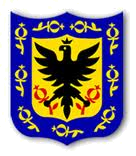
\includegraphics[height=1.75cm]{Images/logo-sed.png} 
\end{minipage}}
\date{}
\begin{document}
\maketitle
Nombre: \hrulefill Curso: \underline{\hspace*{44pt}} Fecha: \underline{\hspace*{2.5cm}}
\begin{enumerate}
\item Ubique en un mismo plano cartesiano los siguientes puntos (2,5) \; (--1,3) \; (3,--2) \; (--2,--4) \; (0,4) \; (0,--5) \; (5,0) \; (--5,0)\\

¿En qué cuadrante se encuentra localizado cada uno de los siguientes puntos?
\begin{multicols}{3}
\item (--5,3)
\item (100,--1)
\item (--6,--29)
\item (3.8,0)
\item $(-\frac{1}{3},0)$
\item $(12\frac{7}{8},-1\frac{1}{2})$
\end{multicols}
¿En qué cuadrante(s) se encuentra localizado el punto descrito?
\item La primera componente ("\emph{abscisa}") es negativa y la segunda componente ("\emph{ordenada}") es positiva
\begin{multicols}{2}
\item La abscisa es positiva
\item La abscisa y la ordenada son iguales
\end{multicols}
\begin{minipage}{.4\textwidth}
\item Encuentre las coordenadas de los puntos $A$, $B$, $C$, $D$ y $E$
\end{minipage}\hfill
\begin{minipage}{.5\textwidth}
\begin{tikzpicture}[scale=.4]
\draw[dotted,style=help lines] (-6,-6) grid (6,6);
\draw[->] (-6,0)--(6,0) node[right] {$x$};
\foreach \x in {1} \draw[shift={(\x,0)},color=black] (0pt,2pt) -- (0pt,-2pt) node[below] {\footnotesize $\x$};
\draw[<->](0,-6)--(0,6)node[left]{$y$};
\foreach \y in {1} \draw[shift={(0,\y)},color=black] (2pt,0)--(-2pt,0) node[left]{\footnotesize $\y$};
\fill (3,3) node[right] {A} circle [radius=.75ex];
\fill (0,-4) node[above right] {B} circle [radius=.75ex];
\fill (-5,0) node[above right] {C} circle [radius=.75ex];
\fill (-1,-1) node[below left] {D} circle [radius=.75ex];
\fill (2,0) node[below right] {E} circle [radius=.75ex];
\end{tikzpicture}
\end{minipage}
\item[C] Determine si la pareja ordenada dada es solución de la ecuación dada
\begin{multicols}{3}
\item (2,9); \; $y=3x-1$
\item (4,2); \ $2x+3y=12$
\item (3,--1); \; $3a-4b=13$
\end{multicols}
En los ejercicios \ref{ej1}--\ref{ej2}, se dan una ecuación y dos parejas ordenadas. Muestre si cada pareja es una solución de la ecuación. Luego encuentre la gráfica de la ecuación para determinar otra solución.
\begin{multicols}{2}
\item $y=x-5$; \; (4,--1) y (1,--4) \label{ej1}
\item $y=\frac{1}{2}x+3$; \; (4,5) y (--2,2)
\item $4x-2y=10$; \; (0,--5) y (4,3)\label{ej2}
\end{multicols}
Grafique cada ecuación e identifique el intercepto con el eje $y$
\begin{multicols}{3}
\item $y=x+1$
\item $y=x$
\item $y=\frac{1}{2}x$
\item $y=x-3$
\item $y=3x-2$
\item $y=\frac{1}{2}x+1$
\item $x+y=-5$
\item $y=\frac{5}{3}x-2$
\item $x+2y=8$
\item $y=\frac{3}{2}x+1$
\item $8x-2y=-10$
\item $8y+2x=-4$
\end{multicols}
\item El número promedio de galones $W$ de agua embotellada consumidos cada año por un norte-americano puede ser aproximado por la ecuación
\[W=1.8d+16.44\]
Donde $d$ es el número de años desde el 2000
\begin{enumerate}
\item Encuentre el número promedio de galones de agua embotellada consumidos en 2001 ($d=1$), en 2010 y en 2015.
\item Grafique la ecuación y use la gráfica para estimar cuál fue el consumo de agua en 2008.
\item ¿En qué año el consumo de agua embotellada será de 36 galones?
\end{enumerate}
Encuentre el valor absoluto de
\begin{multicols}{4}
\item $|-12|$
\item $|0|$
\item $|-3.4|$
\item $|\frac{2}{3}|$
\end{multicols}
\item En años recientes, 2.4\% de los pacientes en los hospitales tenían 75 años de edad. Para un hospital con 200 camas, aproximadamente cuántos pacientes de 75 años habrán?
\item Los puntos (--1,1), (4,1) y (4,--5) son los vertices de un rectángulo. Encuentre las coordenadas del cuarto vértice.
\item Grafique ocho puntos cuya suma de los coordenadas de cada par sea 6
\item Encuentre el perímetro de un rectángulo cuyos vértices tienen las coordenadas $(5,3)$, $(5,-2)$, $(-3,-2)$ y $(-3,3)$.
\end{enumerate}
\end{document}
